\documentclass[12pt, A4paper]{article}
\usepackage{hyperref}
\usepackage{booktabs}
\usepackage{graphicx}
\usepackage{amsmath}
\usepackage[utf8]{inputenc} 
\usepackage{pdflscape}

\usepackage{mhchem}
\usepackage[numbers]{natbib}

\usepackage{fancybox}
\usepackage{graphicx}
\usepackage{color}
%\usepackage[margin=0.7in]{geometry}
\setlength{\abovetopsep}{1em}

\usepackage{siunitx}
\sisetup{locale=ZA}


\usepackage[margin=1.2in]{geometry}

\graphicspath{{graph/}}

\title{CIR310 Phase equilibrium project\\Part 2}
\date{Submission deadline: 22.05.2017 before 13:30}

\newcounter{eqs}
\setcounter{eqs}{0}
\newcommand{\eq}{\stepcounter{eqs}\arabic{eqs}}

\newcounter{variables}
\setcounter{variables}{0}

\newcounter{inputs}
\setcounter{inputs}{0}
\newcommand{\definput}[1]{\ensuremath{#1}\stepcounter{inputs}\stepcounter{variables}}

\newcounter{outputs}
\setcounter{outputs}{0}
\newcommand{\defoutput}[1]{\ensuremath{#1}\stepcounter{outputs}\stepcounter{variables}}

\newcounter{parameters}
\setcounter{parameters}{0}
\newcommand{\defparameter}[1]{\ensuremath{#1}\stepcounter{parameters}\stepcounter{variables}}

\newcommand{\describesection}[1]{\multicolumn{2}{l}{\emph{#1}}}



%% listings
\usepackage{listings}
\usepackage{color}
\definecolor{mygreen}{rgb}{0,0.6,0}
\definecolor{mygray}{rgb}{0.5,0.5,0.5}
\definecolor{mymauve}{rgb}{0.58,0,0.82}
\lstset{ %
  backgroundcolor=\color{white},   % choose the background color; you must add \usepackage{color} or \usepackage{xcolor}; should come as last argument
  basicstyle=\footnotesize,        % the size of the fonts that are used for the code
  breakatwhitespace=false,         % sets if automatic breaks should only happen at whitespace
  breaklines=true,                 % sets automatic line breaking
  captionpos=b,                    % sets the caption-position to bottom
  commentstyle=\color{mygreen},    % comment style
  deletekeywords={...},            % if you want to delete keywords from the given language
  escapeinside={\%*}{*)},          % if you want to add LaTeX within your code
  extendedchars=true,              % lets you use non-ASCII characters; for 8-bits encodings only, does not work with UTF-8
  frame=single,	                   % adds a frame around the code
  keepspaces=true,                 % keeps spaces in text, useful for keeping indentation of code (possibly needs columns=flexible)
  keywordstyle=\color{blue},       % keyword style
  language=Python,                 % the language of the code
  morekeywords={*,...},           % if you want to add more keywords to the set
  numbers=left,                    % where to put the line-numbers; possible values are (none, left, right)
  numbersep=5pt,                   % how far the line-numbers are from the code
  numberstyle=\tiny\color{mygray}, % the style that is used for the line-numbers
  rulecolor=\color{black},         % if not set, the frame-color may be changed on line-breaks within not-black text (e.g. comments (green here))
  showspaces=false,                % show spaces everywhere adding particular underscores; it overrides 'showstringspaces'
  showstringspaces=false,          % underline spaces within strings only
  showtabs=false,                  % show tabs within strings adding particular underscores
  stepnumber=2,                    % the step between two line-numbers. If it's 1, each line will be numbered
  stringstyle=\color{mymauve},     % string literal style
  tabsize=2,	                   % sets default tabsize to 2 spaces
  title=\lstname                   % show the filename of files included with \lstinputlisting; also try caption instead of title
}


\begin{document}
\maketitle
\section{System description}
A coupled reactor/column system is used for trioxane synthesis from formaldehyde to trioxane.  The reversible liquid phase chemical reaction is given by the trimerization reaction:
 
{\centering
\ce{ 3 CH_2O <=>[$[$H^+$]$] C_3H_6O_3 } \par
}
The equilibrium concentration of trioxane is very low in this reaction. A common design solution to increase overall conversion of the process is by using azeotropic distillation with water. A simplified model of this process was developed by \citet{HU19991353}. \autoref{fig:col} demonstrates this process.

 \begin{figure} \centering
 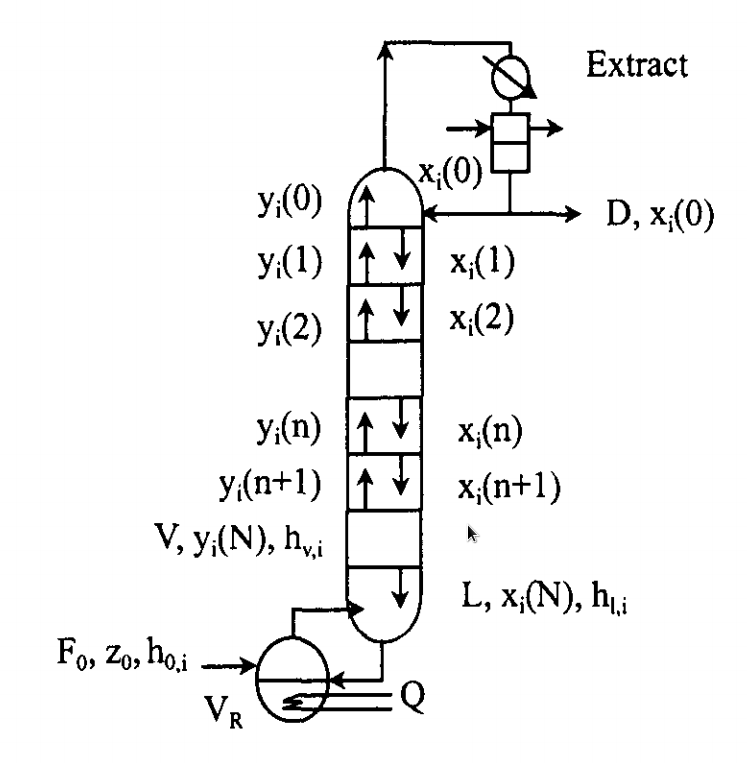
\includegraphics[scale=0.45]{img/reaccol.png}
 \caption{ The coupled reactor/column system (adapted from \citet{HU19991353}).} \label{fig:col}
\end{figure}
 
The feed stream of the reactor contains an aqueous solution of formaldehyde and water.
The goal of the process is to maximise the overall conversion of formaldehyde to trioxane.

\section{Model}
% % Assumptions
The following assumptions have been made for the process.
\begin{enumerate}
\item The entire reactor/column system operates at a continuous steady state equilibrium.
\item The reactor is controlled at a set temperature and the heat transfer dynamics is negligible.
\item The system is adiabatic so that no heat is lost to the environment.
\item The catalytic reaction occurs in the liquid phase of the reactor only. No reaction occurs in the column equilibrium stages.
\item Side reactions and intermediate products are negligible so that the system is a tertiary formaldyhyde-trioxane-water system.
\item A constant relatively volatility is assumed at all stages of the reaction.
\end{enumerate}

The system equations as developed by \citet{HU19991353} are shown in \autoref{tab:equations2}. %A description of parameter, input and output variable names as well as initial steady-state values are presented in Tables~\ref{tab:parameters},~\ref{tab:inputs} and~\ref{tab:outputs}.

%\include{solution_steps}

\begin{landscape}
\begin{table}[htbp]
  \centering
  \caption{System equations. Here $i$ is the chemical component index where $i = 1$ is formaldehyde, $i = 2$  is trioxane and $i=3$ is water. $n$ represents an equilibrium stage $n = 0, 1, 2, \dots N$, the stage $n = N$ is the reactor stage.}
  \label{tab:equations2}
  \begin{tabular}{rllll}
    \toprule
                                  & Equation                                            
                                  & Parameters          
                                  & Inputs         
                                  & Outputs  \\
    \midrule
    \describesection{Reactor mass balance} \\
    \eq                           & $F z_{i} + L x_{i, N} - V y_{i, N} + \upsilon_i r = 0$                           
                                  &   \defparameter{\upsilon_i}
                                  & \definput{F}  \definput{z_{i}}
                                  & \defoutput{ x_{i, N}  }   \defoutput{  y_{i, N}   }  \defoutput{ L }  \defoutput{ V }  \defoutput{  r}    \\
    \describesection{Column mass balance} \\
    \eq                           & $V y_{i, n} - (L + w_i D) x_{i, n} = 0$    
                                  &   \defparameter{w_i}
                                  & \definput{D}
                                  & \defoutput{x_{i, n}}  \defoutput{y_{i, n}} \\
    \eq                           & $L = R D$    
                                  &                       
                                  & \definput{R}
                                  & \\
    \describesection{Component continuity} \\
    \eq                           & $\sum^3_i z_{i} = 1$    
                                  &                       
                                  & 
                                  & \\
    \eq                           & $\sum^3_i x_{i,n} = 1$    
                                  &                       
                                  & 
                                  & \\
    \eq                           & $\sum^3_i y_{i,n} = 1$    
                                  &                       
                                  & 
                                  & \\
    \describesection{Phase equilibrium} \\
    \eq                           & $ \alpha_i = \frac{ y_{i,n} / y_{1, n} }{ x_{i, n+1} / x_{_{1, n + 1}} } $    
                                  &                       
                                  & 
                                  & \defoutput{\alpha_i} \\
    \describesection{Reaction rate equation} \\
    \eq                           & $ r = V_r \left( k_1 C_1^2 - k_2 C_2 \right)  $    
                                  &  \defparameter{k_1} \defparameter{k_2}       
                                  & 
                                  & \defoutput{r}\\
    \describesection{Energy balance} \\
    \eq                           & $ \sum^3_i \left[ Fz_i h_{F, i} + L x_{i, N} h_{l, i} - V y_{i, N} h_{v, i} \right] + Q = 0$    
                                 &                       
                                  & \definput{ h_{F, i} } \definput{ h_{l, i} } \definput{ h_{v, i} } \definput{ Q }
                                 & \\
    \midrule
                                  & Total: \arabic{variables} = & \arabic{parameters} & +\arabic{inputs} & +\arabic{outputs}  \\
    \bottomrule
  \end{tabular}
\end{table}

\end{landscape}



\section{Instructions}

Based on your findings from the initial investigation into the process model it was decided that a more sophisticated thermodynamic model would be required to accurately simulate this system. You and your team have been directed to incorporate a cubic equation of state model with appropriate mixing rule parameters into the model. To calculate the fugacities from the mechanical equation of state (a PVT relation) we will need to find expressions for the fugacity coefficients of a component in a mixture. We can then use the set of equations
 $$y_i \hat{\phi}_i^v  - x_i \hat{\phi}_i^l = 0$$ for all $i = 1, 2, 3 $
 to replace the phase equilibrium equations in the system of equations from \autoref{tab:equations2} at every equilibrium stage in the column.

\subsection{Symbolic computations}
The fugacity coefficient of a component $i$ in a mixture can be calculated using Equation 11.60 from Smith, Van Ness and Abbott \citep[p. 404]{smith2005introduction} 
\begin{equation} \label{eq:phi_i}
\ln{\hat{\phi}_i} = \int^P_0 (\bar{Z}_i - 1) \frac{d P}{P}
\end{equation}
where $\bar{Z}_i  = \frac{\left( \partial n Z \right)}{\partial n_i}$. Using this equation together with the Van der Waals mixing parameters. \citep[p. 561,  Equations 14.42 and 14.43]{smith2005introduction})
\begin{equation} \label{eq:b_mix}
b = \sum_{i} x_i b_i
\end{equation}

\begin{equation} \label{eq:a_mix}
a = \sum_{i}\sum_{j} x_i x_j a_{ij}
\end{equation}
 where $a_{ij} = \sqrt{a_i a_j}$. Using these three equations derive the following expressions.


\begin{enumerate}
\item 
%% VdW
The van der Waals equation of state is given by
\begin{equation}
P = \frac{RT}{v - b} - \frac{a}{v^2}
\end{equation}
 Show that the fugacity coefficient of component $i$ in a mixture described by the Van der Waals equation of state is given by
  
\begin{equation}
\ln{\hat{\phi}_i} = \ln{\left(\frac{v}{v - b} \right)}+ \frac{b_i}{v - b} - \frac{2 \sqrt{a_i} \sum_{i = 1}^n x_i \sqrt{a_i} }{v R T} - \ln{Z}
\end{equation}
 
  \textit{HINT: You can change the variable of integration of \autoref{eq:phi_i} with the identity:  $\frac{dP}{P} = \frac{dZ}{Z} - \frac{dV}{V}$  (derive this from $Z = \frac{PV}{RT}$)}.
  
 %\textit{HINT 2: It might be useful to rewrite the EOS in its explicit compressibility form first.}
  
   
   
\begin{flushright} 
\Ovalbox{30}
\end{flushright}
%\item
%%PR
%The Peng-Robinson equation of state is given by
%\begin{equation}
%P = \frac{RT}{v - b} - \frac{a }{ v(v + b) + b (v - b)}
%\end{equation}

 %Show that the fugacity coefficient of component $i$ in a mixture described by the Peng-Robinson equation of state is given by
 
%\begin{equation}
%\ln{\hat{\phi}_i} = \frac{b_i}{b} (z - 1) - \ln{\left( Z - \frac{b P}{RT} \right) - \frac{a}{2 \sqrt{2} b R T} \left(\frac{2 \sum_{j} y_j a_{ij}}{a} - \frac{b_i}{b} \right) \ln{\left( \frac{ v + b \left( 1 + \sqrt{2}\right) }{v + b \left( 1 - \sqrt{2}\right) }\right)}}
%\end{equation}
%\begin{flushright} 
%\Ovalbox{35}
%\end{flushright}

\item
 %% RK 
 The Redlich-Kwong (RK) equation of state is given by
\begin{equation}  \label{eq:RK}
 P = \frac{RT}{v - b} - \frac{a}{\sqrt{T} v \left(v + b \right)}
\end{equation}

 Show that the fugacity coefficient of component $i$ in a mixture described by the Redlich-Kwong equation of state is given by
\begin{equation} \label{eq:phi_RK}
\ln{\hat{\phi}_i} = \ln{\left(\frac{v}{v - b} \right)}  + \frac{b_i}{v - b} - \frac{2 \sum_{j} y_j a_{ji}}{R T^{3/2} b} \ln{\left( \frac{v + b}{v} \right)}  + \frac{a b_i}{RT^{3/2} b^2} \left( \ln \left( \frac{v + b}{v}\right) \frac{b}{v + b}  \right) - \ln Z
\end{equation} 
\begin{flushright} 
\Ovalbox{50}
\end{flushright}

\item Rewrite the RK-EOS given in \autoref{eq:RK} in cubic form ($\dots v^3 + \dots v^2 +\dots v  + \dots = 0 $) and show how the roots of this equation depend on the composition of the mixture. Describe how you would calculate a liquid and a vapour root.

\begin{flushright} 
\Ovalbox{20}
\end{flushright}

\end{enumerate}

\begin{centering}
Total Marks: \Ovalbox{100}\\
\end{centering}

\subsection{Numerical computations}
Write the functions to work for system consisting of an arbitrary amount of components, but use the compounds and their associated parameters of the ternary system described in this project to test your code. For all these questions you may use the functions you've already developed in subsequent questions. You may assume that the pure component parameters are global parameters (ex. $a_i$, $b_i$ and $R$).
\begin{enumerate}
\item  Write two functions that accepts a vector of compositions as an input and returns the $a_{mix}$ and $b_{mix}$ parameters defined by \autoref{eq:a_mix} and \autoref{eq:b_mix}. Assume that the pure component parameters are global variables in your code.  Suggested format:
   
\begin{lstlisting}
def a_mix(x):
    ...
    return a_mix
\end{lstlisting}

\begin{lstlisting}
def b_mix(x):
    ...
    return  b_mix
\end{lstlisting}

\begin{flushright} 
\Ovalbox{15}
\end{flushright}

\item  Write two functions that accepts as an input the pressure, temperature and compositions states of a mixture calculates a vapour and liquid root of the RK-EOS  \autoref{eq:RK} at the input composition.
   
\begin{lstlisting}
def V_l(P, T, x):
    ...
    return V_l
\end{lstlisting}

\begin{lstlisting}
def V_v(P, T, x):
    ...
    return  V_v
\end{lstlisting}

\begin{flushright} 
\Ovalbox{30}
\end{flushright}

\item  Write a function that calculates the fugacity coefficient of a component $i$ in in a mixture described by the RK-EOS  \autoref{eq:phi_RK} for an arbitrary phase $\theta$ with it's associated volume root $v^\theta$.
   
\begin{lstlisting}
def phi_i_theta(P, T, x, i, v_theta):
    ...
    return  phi_i_theta
\end{lstlisting}

\begin{flushright} 
\Ovalbox{30}
\end{flushright}

\item Remembering that the temperature of the system is a specified input and further assume that P is constant at one atmosphere. Assume that there are only two phases (a liquid and a vapour phase). Write a function that accepts an input a vector of composition variables and outputs the residual of the equations $$y_i \hat{\phi}_i^v  - x_i \hat{\phi}_i^l = 0$$ for all $i = 1, 2, \dots N $. The function should wrap the previous functions and accept as an input a single vector of dimensions $2 \times N $ containing all compositions (which can be used in a non-linear solver) and output the results of the functions of  $N$

\begin{lstlisting}
N = 3  # 3 components
def solver(X):  # For N = 3, X is a vector representing 
	  	   			  # X = [x_1, x_2, x_3, y_1, y_2, y_3]
    x = X[0:N]  # A vector of liquid phase compositions
    y = X[N:]   # A vector of vapour phase compositions
    ...
    return F_PHI  # A vector of N outputs of the equations
\end{lstlisting}

\begin{flushright} 
\Ovalbox{25}
\end{flushright}

\end{enumerate}

 
\begin{centering}
Total Marks: \Ovalbox{100}\\
\end{centering}

%\pagebreak
\bibliographystyle{apalike}
%\bibliographystyle{spmpsci}
\bibliography{lib}

\end{document}
